\chapter[Statistics, and Probability]{Problem-Solving Strategies for Data Analysis, Statistics, and Probability}

\subsection{SAT Worksheet 1G: Warm-Up Problems}

\textbf{Strategies and content practice:} Write which strategy or strategies that you want to use to solve the following word problems. Then, solve the problem.

\begin{multienumerate}
\mitemxx{\medium

Maria makes a bet with her friends that if she pulls two cards out of a deck without replacing them, the first will be a red number card (2-10) and the second will be a black face card (Jack, Queen, King, Ace). What are the odds of Maria winning this bet?

\begin{enumerate}[label=(\Alph*)]
\item 12/221
\item 9/169
\item 11/26
\item 25/102
\item 13/200
\end{enumerate}}{\medium

If a fair six-sided dice is rolled twice and predictions are made on the outcome. Which of the following predictions has the highest chance of being true?

\begin{enumerate}[label=(\Alph*)]
\item Five will be rolled twice
\item An even number will be rolled first and an odd number will be rolled second
\item Two even numbers will be rolled
\item The sum of the two numbers will be either 8 or 9
\item The sum of the two numbers will be less than 7
\end{enumerate}}

\vfill
\mitemxx{\advanced

Marcus has recently been told by his doctor that he should try to eat one fruit, one vegetable, and one meat every day. For fruit, Marcus loves strawberries, bananas, and blueberries. For vegetables he only likes corn and carrots. For meat, Marcus enjoys chicken, beef, pork, and lamb. If Marcus tries a different combination every day of fruit, vegetables, and meat, how many possible combinations will be available to pick from on the beginning of the fifth day?}{\advanced

What is the greatest number of pieces that can be made from a cylinder using only three cuts (without moving any of the pieces)?

\begin{enumerate}[label=(\Alph*)]
\item 5
\item 6
\item 7
\item 8
\item 9
\end{enumerate}}
\end{multienumerate}

\newpage
\section[Visual Data]{Visual Data, Data Analysis, and Statistics}

Examples:

\centerline{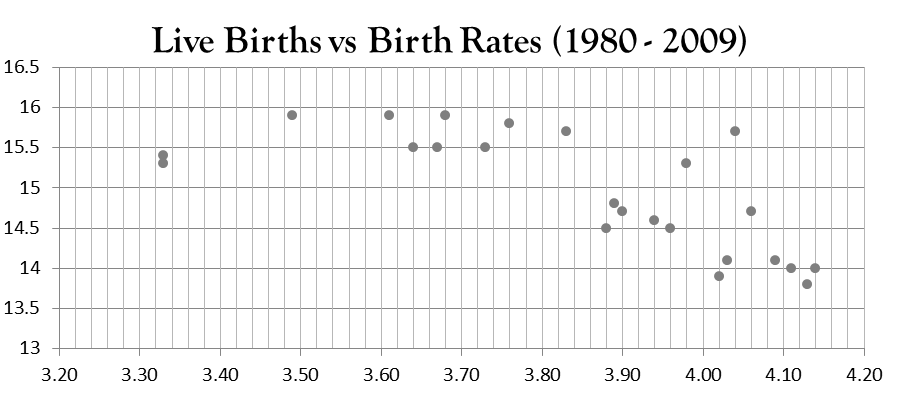
\includegraphics{56}}

\begin{multienumerate}
\mitemxx{\basic

The graph above represents the number of live births (in millions) versus the birth rates (number of births per 1000 in a population) in the US from 1980 to 2009. Which of the following is not likely to be a point on the graph?

\begin{enumerate}[label=(\Alph*)]
\item $(3.3,20)$
\item $(3.8,15)$
\item $(3.9,14.3)$
\item $(4.1,16)$
\item $(4.2,16.5)$
\end{enumerate}}{\medium

Which of the following statements can be inferred by the information on the graph above?

\begin{enumerate}[label=(\Alph*)]
\item Birth rates are decreasing every year
\item The number of live births are increasing every year
\item The birth rate is decreasing as the number of live births is increasing
\item The total population in the US is decreasing every year
\item More families are adopting every year
\end{enumerate}}
\end{multienumerate}

\hrulefill

The SATS will include summaries of data in the form of tables, charts, and graphs.

\begin{itemize}
\item Basic questions will ask to you to find information from the visual given. Oftentimes, you will need to perform a basic operation on the numbers that you are pulling from the data, such as adding products from one year to another year or converting the percentages on a circle graph (pie chart) to actual numbers.
\vfill\item More difficult questions can be difficult for the following reasons: 1) The question asks you to perform a more complicated operation based on information given the visual or 2) The question or the visual data includes a component that is extremely tricky. See some of the tricks used (and how to avoid them) in the strategy section below.

\textbf{Strategies for surviving the visual data and data analysis section}

\item Strategy \#1: Read the written information. This may include the main title, the $x$-axis title, and the $y$-axis title. \textit{Pay particular attention to the scaling information found immediately after the titles. It is possible (and probable on the more difficult problems) that the $x$- and $y$-axes will have different scaling.}

\vfill
\item Strategy \#2: When a question is asked about percent increase or decrease, remember that the change is relative. This means that in a bar graph, a relatively small bar becoming only slightly smaller might still be a larger percentage increase than a huge bar turning into a smaller bar. Why does this phenomenon occur? (Hint: think about the general equation for percentage increase or decrease.) \hrulefill

\vfill
\item Strategy \#3: Identify what you are solving for in the question before you solve the problem, and after you have solved for an answer, check to make sure that your answer actually represents what you were asked to solve for in the question.
\end{itemize}

\vfill
\newpage
\subsection{SAT Worksheet 2G: 6 Questions, 8 Minutes}

\begin{enumerate}
\centerline{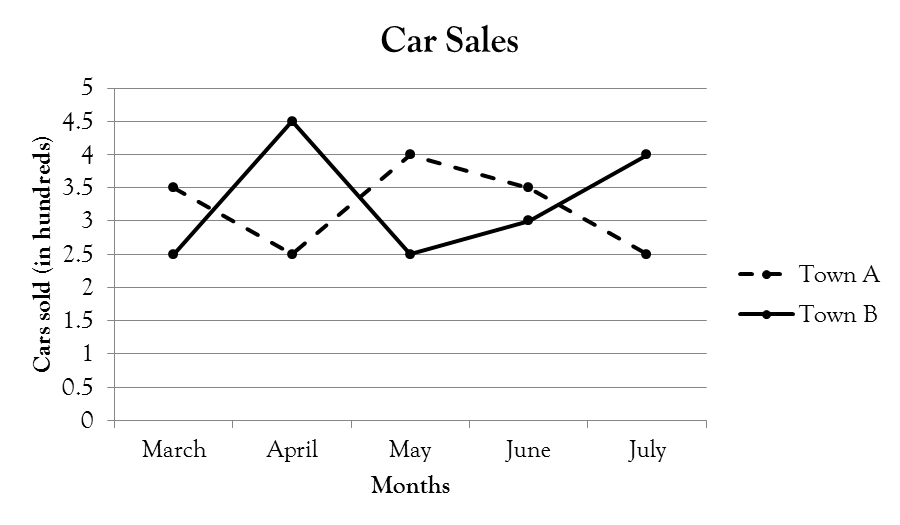
\includegraphics{57}}

\item \basic

The chart above shows the car sales of Town A and Town B over a four month span. During which month is the difference between the car sales in each town the greatest?

\begin{enumerate}[label=(\Alph*)]
\item March
\item April
\item May
\item June
\item July
\end{enumerate}

\vfill
\item \basic

How many more cars were sold in Town B than Town A during the month of July?

\begin{enumerate}[label=(\Alph*)]
\item 15
\item 100
\item 150
\item 1,000
\item 1,500
\end{enumerate}

\newpage
\centerline{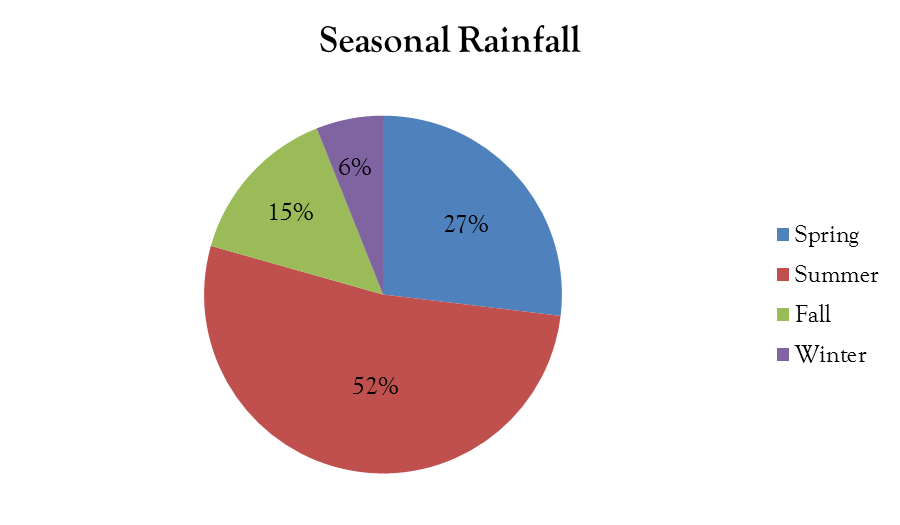
\includegraphics{58}}

\item \medium

Above is a chart of the average (arithmetic mean) seasonal rainfall in Colorado Springs. If the total annual rainfall is 16.54 inches, what is the average amount, in centimeters, of rainfall in the winter?

\begin{enumerate}[label=(\Alph*)]
\item 1 cm
\item 2 cm
\item 4 cm
\item 5 cm
\item 6 cm
\end{enumerate}

\vfill
\newpage
\centerline{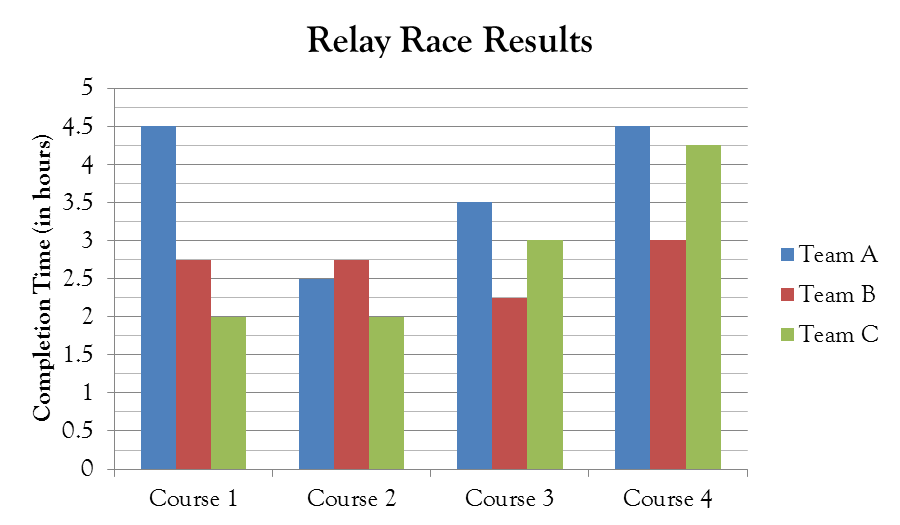
\includegraphics{59}}

\item \medium

Three teams competed in a relay race. How many more minutes did Team B take than Team C on Course 2?

\begin{enumerate}[label=(\Alph*)]
\item 25\%
\item 33\%
\item 75\%
\item 125\%
\item 133\%
\end{enumerate}

\vfill
\item \advanced

In what percent did the average time of Team C complete in the average time of Team A?

\begin{enumerate}[label=(\Alph*)]
\item 25\%
\item 33\%
\item 75\%
\item 125\%
\item 133\%
\end{enumerate}

\vfill
\newpage
\centerline{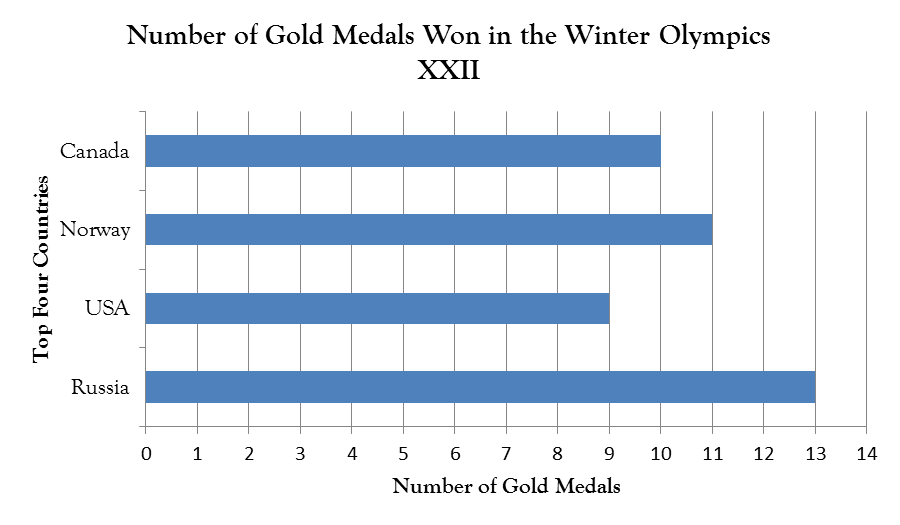
\includegraphics{60}}

\item \advanced

Above is a chart with the countries that received the most number of gold medals in the Winter Olympics XXII. Approximately what percentage of gold medals was won by the two lowest performing countries relative to the top two? (Round to the nearest whole number)

\begin{enumerate}[label=(\Alph*)]
\item 38\%
\item 44\%
\item 69\%
\item 77\%
\item 79\%
\end{enumerate}
\end{enumerate}

\newpage
\section{Averages}

We reviewed the basic formula for averages in the chapter about strategies for algebra, but given that it is a difficult topic, we will discuss it in more depth here. The general formula for averages is:

\vfill
Examples:

\begin{multienumerate}
\mitemxx{\basic

Set A contains $x$ positive integers. If the average (arithmetic mean) is 10, which expression represents their sum?

\begin{enumerate}[label=(\Alph*)]
\item $10-x$
\item $10+x$
\item $10x$
\item $x/10$
\item $10/x$
\end{enumerate}}{\medium

The average (arithmetic mean) of five consecutive even integers is 20. What is the value of the median?

\begin{enumerate}[label=(\Alph*)]
\item 8
\item 10
\item 14
\item 16
\item 20
\end{enumerate}}
\end{multienumerate}

\hrulefill

The more complicated SAT problems on averages usually have to do with solving for\ldots

\textbf{A part of the sum (the numerator of the equation)}- you can do this by using a variable like $x$ to represent the unknown part of the sum and then get $x$ by itself.

\vfill
\textbf{Finding weighted averages}- The average of 50 and 60 is 55 (the middle). However, when you take the average of 50, 60, and 60, the average is closer to \shortline than 60. As a result, you can take into account the number of occurrences weighted by the value of each unique occurrence. This answer will be your sum that can be plugged into the averages formula. 

\vfill
\textbf{The average from visual data}- Here you will find the number of occurrences weighted by the value of each unique occurrence from the chart. Then, solve using the strategy presented in the``finding weighted averages'' category above. 

\vfill
\newpage
\subsection{SAT Worksheet 3G: 6 Questions, 8 Minutes}

\begin{multienumerate}
\mitemxx{\basic The average of $k, k+4$, and $k+8$ is 15. What is the value of $k$?

\begin{enumerate}[label=(\Alph*)]
\item 10
\item 11
\item 15
\item 19
\item 33
\end{enumerate}}{\basic

If the average (arithmetic mean) of 5 numbers is 20, then what is the value of their sum?

\begin{enumerate}[label=(\Alph*)]
\item 15
\item 20
\item 25
\item 50
\item 100
\end{enumerate}}

\vfill
\mitemxx{\medium

Debbie has taken four tests, receiving 78\%, 83\%, 92\%, and 81\%. What grade must she receive on her fifth test in order to have an average of 85\% or better overall?

\begin{enumerate}[label=(\Alph*)]
\item 84\%
\item 85\%
\item 87\%
\item 91\%
\item 92\%
\end{enumerate}
}{\medium

If a set contains five non-negative integers and the average is even, what is the most amount of odd numbers that the set can contain?

\begin{enumerate}[label=(\Alph*)]
\item 0
\item 1
\item 2
\item 3
\item 4
\end{enumerate}}

\vfill
\mitemxx{\advanced

For two positive integers $a$ and $b$, the average of their squares is equal to the square of their average. Which of the following must be true?

\begin{enumerate}[label=\Roman*.]
\item $ab$ is also a perfect square
\item $a=b$
\item $a/b=1$
\end{enumerate}

\begin{enumerate}[label=(\Alph*)]
\item I only
\item II only
\item III only
\item I and III only
\item I, II, and III
\end{enumerate}}{\advanced

\begin{enumerate}[label=\Roman*.]
\item The median of set A is greater than the median of set B
\item The sum of the numbers in set A is smaller than the sum of the numbers in set B
\item Set A shares at least one number in common with set B
\end{enumerate}

\begin{enumerate}[label=(\Alph*)]
\item I only
\item II only
\item III only
\item I and III only
\item I, II, and III
\end{enumerate}}
\end{multienumerate}

\newpage
\subsection{SAT Worksheet 4G (Basic): 5 Questions, 7 Minutes}

\begin{multienumerate}
\centerline{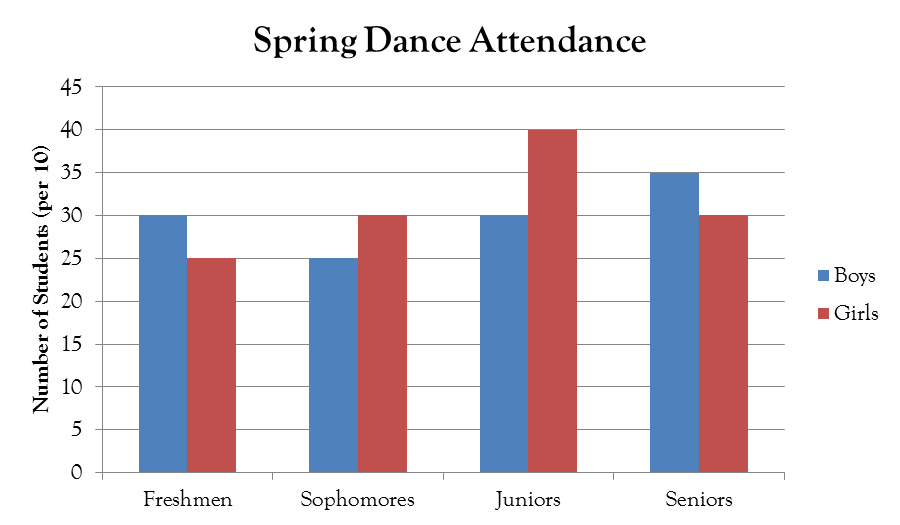
\includegraphics{61}}

\mitemx{The chart above shows the number of students attending the spring dance by class year and gender. How many more girls attended the dance than boys?

\begin{enumerate}[label=(\Alph*)]
\item 5
\item 15
\item 25
\item 30
\item 50
\end{enumerate}}

\vfill
\mitemxx{The sum of 6 numbers is $42m+18n$. What is their average (arithmetic mean)?

\begin{enumerate}[label=(\Alph*)]
\item $7m+3n$
\item $7n+3m$
\item $7m-3n$
\item $36m+12n$
\item $48m-24n$
\end{enumerate}}{Which of the following sets has an average of $2n+1$?

\begin{enumerate}[label=(\Alph*)]
\item ${n-2, n-1, n}$
\item ${n-1, n, n+1}$
\item ${n, n+1, n+2}$
\item ${2n, 2n+1, 2n+2}$
\item ${3n, 3n+2, 3n+4}$
\end{enumerate}}
\end{multienumerate}

\vfill
\newpage
\centerline{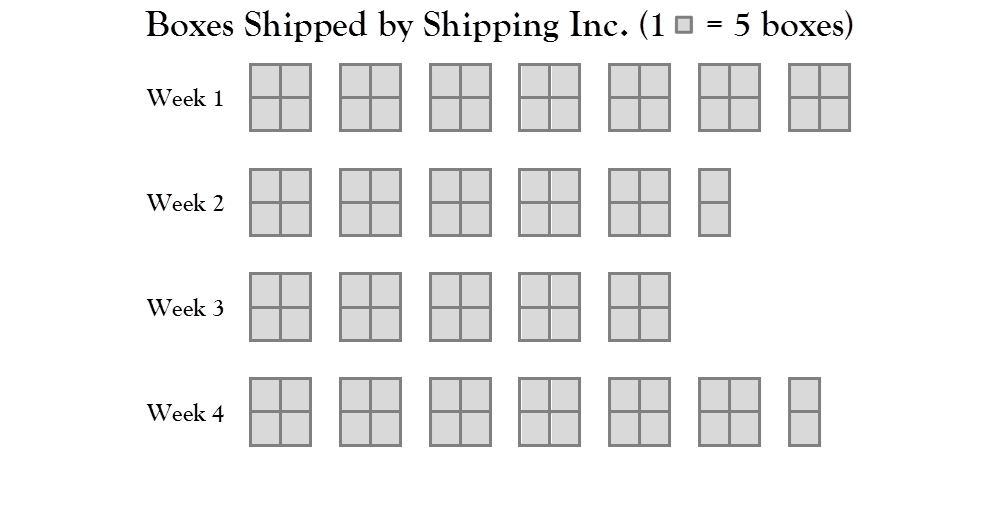
\includegraphics{62}}

\begin{multienumerate}
\mitemx{The graph above indicates the number of boxes shipped by Shipping Inc. over four weeks. How many boxes were shipped during week 2?

\begin{enumerate}[label=(\Alph*)]
\item 5.5
\item 30
\item 55
\item 110
\item 120
\end{enumerate}}

\vfill
\mitemx{The average of three positive integers is even. Which of the following must be true?

\begin{enumerate}[label=\Roman*.]
\item The three integers must be even
\item The sum of the three integers must be even
\item Each of the integers must be divisible by three
\end{enumerate}

\begin{enumerate}[label=(\Alph*)]
\item I only
\item II only
\item III only
\item I and II only
\item I, II, and III
\end{enumerate}}
\end{multienumerate}

\vfill
\newpage
\subsection{SAT Worksheet 5G (Medium): 7 Questions, 10 Minutes}

\begin{multienumerate}
\mitemxx{Roberta flips a penny 20 times, landing on heads a total number of 8 times. She flips the same penny another 30 times, landing on heads 21 times. What is the overall average percentage of times the penny landed tails?

\begin{enumerate}[label=(\Alph*)]
\item 40\%
\item 45\%
\item 50\%
\item 55\%
\item 60\%
\end{enumerate}}{

\medskip
\begin{tabular}{|l|c|c|c|}\hline
\multicolumn{4}{|c|}{Approximate Conversions}\\\hline
Number of Inches & 1.2 & 2.4 & 4.8\\\hline
Number of Centimeters & $x$ & 6.1 & 12.2\\\hline
\end{tabular}

\medskip
The table above shows the approximate conversions from inches to centimeters. What is the approximate value of $x$?

\begin{enumerate}[label=(\Alph*)]
\item 1.53
\item 2.54
\item 3.05
\item 3.50
\item 2.87
\end{enumerate}}

\vfill
\mitemxx{Ms. Miller found the average height of her students to be exactly 56 inches tall. If the class consisted of 10 students and the shortest student was a height of 42 inches, what is the lowest possible value for the height of the tallest student?

\begin{enumerate}[label=(\Alph*)]
\item 56.5 in
\item 57.6 in
\item 59.5 in
\item 70.5 in
\item 72.1 in
\end{enumerate}}{If the largest number in a set is equal to the average (arithmetic mean) of the set, which of the following must be true?

\begin{enumerate}[label=\Roman*.]
\item The median is equal to the average
\item The smallest number is equal to the largest number
\item The set contains only one number
\end{enumerate}

\begin{enumerate}[label=(\Alph*)]
\item I only
\item II only
\item III only
\item I and II only
\item I, II, and III
\end{enumerate}}

\vfill
\newpage
\centerline{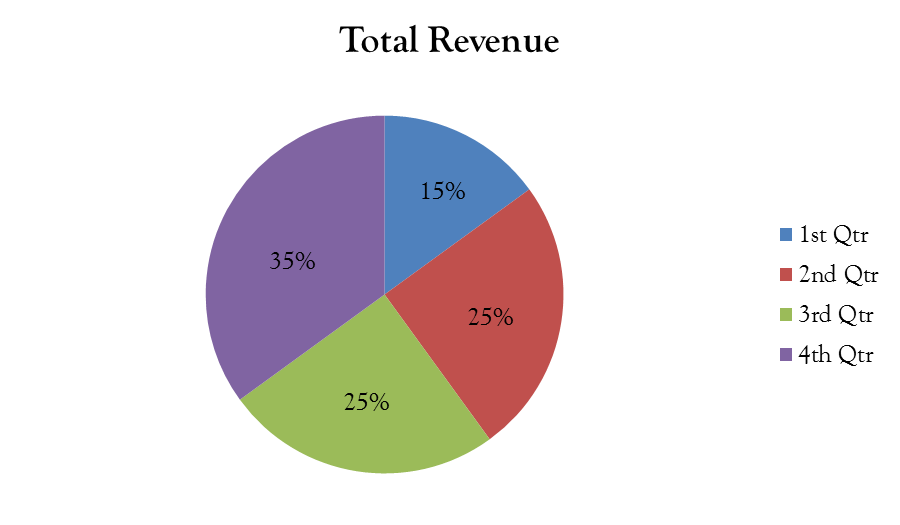
\includegraphics{63}}

\mitemx{What ratio of the total revenue was brought by the first and second quarter?

\begin{enumerate}[label=(\Alph*)]
\item $2:5$
\item $3:5$
\item $2:3$
\item $1:2$
\item $4:5$
\end{enumerate}}

\vfill
\mitemx{The following graph represents the revenue of Cheerful Toys last year. If the first and second quarter combined yielded a profit of \$200,000, how much revenue was brought in the third and fourth quarter combined?

\begin{enumerate}[label=(\Alph*)]
\item 100,000
\item 200,000
\item 300,000
\item 400,000
\item 500,000
\end{enumerate}}

\vfill
\newpage
\centerline{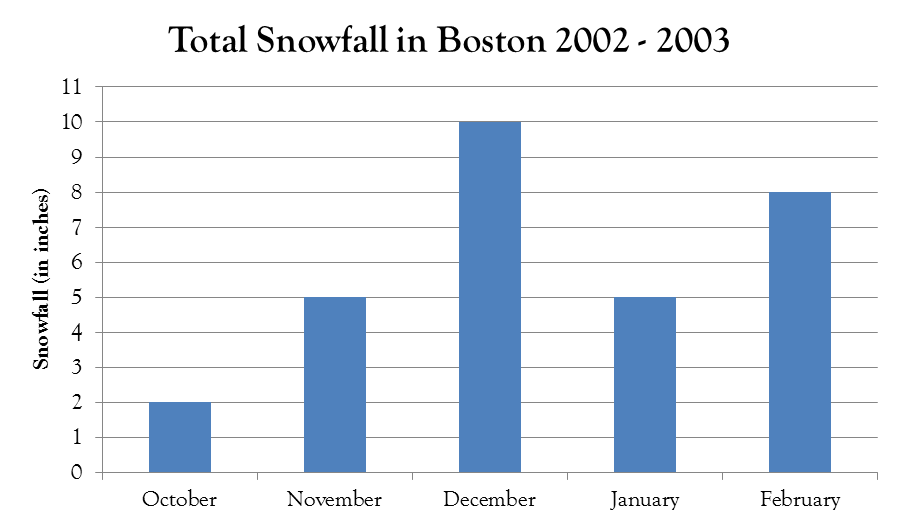
\includegraphics{64}}

\mitemx{The chart above indicates the total snowfall in Boston during the winter of 2002-2003. Which interval below indicates the greatest rate of increase in snowfall?

\begin{enumerate}[label=(\Alph*)]
\item October to December
\item November to December
\item January to February
\item November to February
\item October to February
\end{enumerate}}
\end{multienumerate}

\vfill
\newpage
\subsection{SAT Worksheet 6G (Advanced): 6 Questions, 10 Minutes}

\begin{multienumerate}
\mitemxx{The average (arithmetic mean) of 1, 3, $x$, 5, and 9 is 4. The average (arithmetic mean) of 2, 4, $y$, 8, and 10 is 6. What is the value of $xy$?

\begin{enumerate}[label=(\Alph*)]
\item 5
\item 8
\item 10
\item 11
\item 12
\end{enumerate}}{The average (arithmetic mean) of 6 numbers is 6. When a seventh number is added, the average is 8. What number was added?

\begin{enumerate}[label=(\Alph*)]
\item 20
\item 30
\item 40
\item 50
\item 60
\end{enumerate}}

\centerline{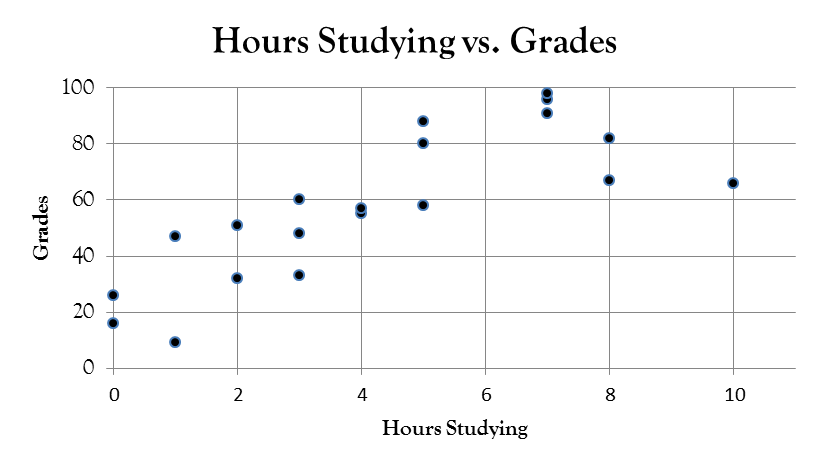
\includegraphics{65}}

\mitemx{The graph above compares the number of hours students spent studying versus the grades received on their final exam. How many students studied 5 hours or more and received a score of less than 70\%?

\begin{enumerate}[label=(\Alph*)]
\item 1 student
\item 2 students
\item 3 students
\item 4 students
\item More than 4 students
\end{enumerate}}

\newpage
\centerline{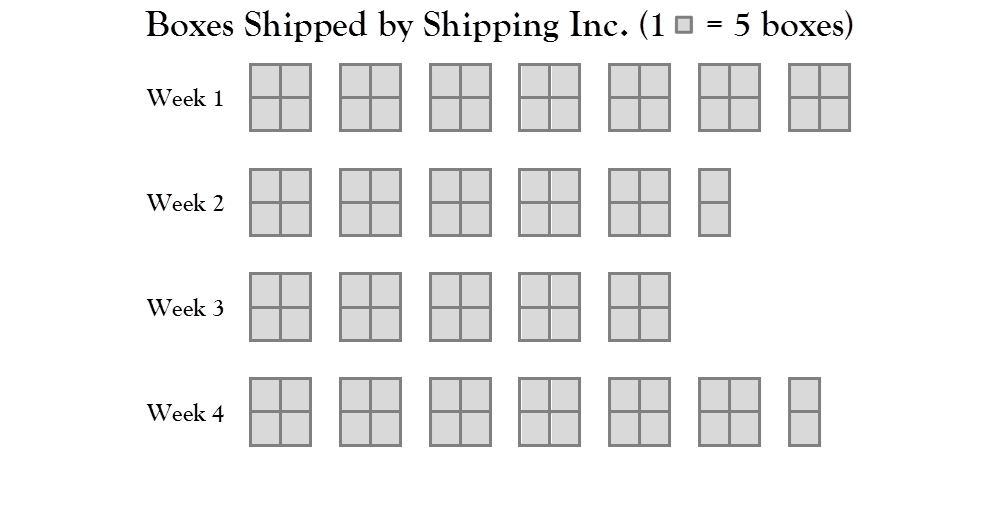
\includegraphics{66}}

\mitemx{What is the greatest difference between the average (arithmetic mean) and the least number of boxes shipped in a week?

\begin{enumerate}[label=(\Alph*)]
\item 20
\item 40
\item 50
\item 60
\item 80
\end{enumerate}}

\vfill
\mitemxx{Which of the following is the sum of three consecutive odd integers?

\begin{enumerate}[label=(\Alph*)]
\item 32
\item 33
\item 34
\item 35
\item 36
\end{enumerate}}{The average (arithmetic mean) of five consecutive integers is 3 times more than the median, $c$. Which of the following statements must be true?

\begin{enumerate}[label=\Roman*.]
\item The median is 0
\item The average is 0
\item The sum of the five consecutive integers is 0
\end{enumerate}

\begin{enumerate}[label=(\Alph*)]
\item I only
\item II only
\item III only
\item I and III only
\item I, II, and III
\end{enumerate}}
\end{multienumerate}
